\section{Metodologia}\label{sec:metodologia}

Nesta seção será apresentada a metodologia de pesquisa e experimentação. Na Seção~\ref{subsec:dataset} serão descritos os conjuntos de dados utilizados e nas Sessões~\ref{subsec:metricas},~\ref{subsec:algoritmos} e~\ref{subsec:experimentos} e serão expostos detalhes sobre as métricas para avaliação, técnicas de extração utilizadas e os experimentos realizados, respectivamente.


\subsection{Conjuntos de dados}\label{subsec:dataset}

Foi feita uma pesquisa por conjuntos de dados públicos para a realização de treinamento e teste de modelos para extração de características. A seguir, uma breve descrição sobre os conjuntos de dados encontrados.


\subsubsection{\textit{Fingerprint Verification Competition} (FVC)}\label{subsubsec:fvc}

Foram realizadas algumas competições organizadas por pesquisadores da \textit{University of Bologna} para avaliação de sistemas de reconhecimento de usuários pela impressão digital. As partes A e B dos conjuntos de dados utilizados nas edições de 2000, 2002 e 2004 foram disponibilizadas publicamente como um material adicional da publicação de~\citeonline{handbook_of_fp_recognition}.

Para cada ano da competição, há 4 conjuntos de dados, sendo 3 deles coletados com diferentes sensores e um quarto conjunto de impressões digitais sintéticas geradas através do software SFinGe~\cite{handbook_of_fp_recognition}. Cada um deles foi separados nas partes ``A'', com imagens de 100 dedos, e ``B'', com imagens de 10 dedos. Para cada dedo há 8 impressões digitais, totalizando 880 imagens em cada conjunto. Portanto, no total, o FVC possui $880 \times 4 \times 3 = 10560$ imagens.


\subsubsection{Neurotechnology}\label{subsubsec:neurotechnology}

A empresa Neurotechnology disponibilizou dois conjuntos de imagens de impressão digital, que podem ser acessados pelo site~\footnote{\url{https://www.neurotechnology.com/download.html}}. O primeiro conjunto de dados possui imagens de $51$ dedos com $8$ impressões cada, totalizando $408$ imagens capturadas com o leitor~\textit{Cross Match Verifier 300}. O segundo possui imagens de $65$ dedos com 8 impressões cada, totalizando 520 imagens coletadas com o leitor~\textit{DigitalPersona U.are.U 4000}.


\subsection{Métricas}\label{subsec:metricas}

Esta seção descreve algumas métricas usadas na literatura que serão usadas para avaliação dos resultados nos experimentos realizados neste projeto de pesquisa. Essas métricas são: FMR, FNMR e acurácia balanceada~\cite{Precise2014, Ferlini2021eargate}. Uma breve descrição dessas métricas é apresentadas a seguir:

\begin{itemize}
    \item FMR (\textit{False Match Rate}, Taxa de falsa correspondência): percentual de tentativas de impostores que foram aceitas como genuínas, definida como

        \begin{equation}\label{eqn:fmr}
            FMR = \frac{número\:de\:tentativas\:de\:impostores\:aceitas}{total\:de\:tentativas\:de\:impostores}.
        \end{equation}

        Uma taxa relacionada é a FAR (\textit{False Acceptance Rate}), que tem significado similar, mas considera também taxa em que o sistema biométrico falha ao obter uma amostra biométrica. Essa taxa é conhecida como FTA (\textit{Failure to Acquire Rate}).


    \item FNMR (\textit{False Non-match Rate}, Taxa de falsa não-correspondência): percentual de tentativas genuínas que foram rejeitadas como impostoras pelo sistema, definida como

        \begin{equation}\label{eqn:fnmr}
            FNMR = \frac{número\:de\:tentativas\:genuínas\:rejeitadas}{total\:de\:tentativas\:de\:usuários\:genuínos}.
        \end{equation}

        Uma métrica relacionada é a FRR (\textit{False Rejection Rate}), que tem um significado similar, mas considera também a FTA.

    \item Acurácia balanceada: média do acerto para cada classe (genuíno e impostor). Essa métrica pode ser obtida a partir do cálculo da (HTER -~\textit{Half Total Error}, Metade do erro total)
          
        \begin{equation}\label{eqn:hter}
            HTER = \frac{FNMR + FMR}{2},
        \end{equation}

        definida como a média entre FNMR e FMR~\cite{Roy2022systematic}. A partir da HTER, então é obtida a acurácia balanceada,

        \begin{equation}\label{eqn:bacc}
            BAcc = 1 - HTER.
        \end{equation}
    
    \item EER (\textit{Equal Error Rate, Taxa de erro igual}): ponto em que a FMR é igual a FNMR, em um determinado limiar de corte. 

\end{itemize}


\subsection{Algoritmos}\label{subsec:algoritmos}

Para os experimentos iniciais foram feitas buscas por repositórios com código-fonte disponíveis publicamente ou modelos pré-treinados que poderiam ter sido disponibilizados pelos autores dos artigos lidos na revisão bibliográfica. Foram feitos experimentos com o modelo {DeepPrint} implementado por~\citeonline{Rohwedder2023} e com o FLARE, implementado pelos próprios autores.


\subsubsection{Arquitetura do~\textit{DeepPrint}}\label{subsubsec:deepprint-arch}

\citeonline{deep_print} desenvolveram uma Rede Neural Convolucional (\textit{Convolutional Neural Network} ou CNN) que ``aprende'' a extrair uma representação de tamanho fixo (um vetor) a partir de uma impressão digital. Como entrada a rede recebe uma imagem de tamanho $448 \times 448$ em escala de cinza (cada pixel assume um valor de 0 a 255) e passa primeiro pelo módulo de alinhamento. O módulo de alinhamento utiliza uma rede neural de transformação espacial~\cite{spatial-transformer-networks} para fazer com que a impressão digital na imagem fique no centro. 

Em seguida, a imagem passa por uma rede base, que consiste na parte inicial da arquitetura \textit{Inception} v4~\cite{inception-v4}, isso é, sem os módulos~\textit{Inception}. Neste ponto a rede é bifurcada em duas novas redes. A primeira completa a arquitetura da~\textit{Inception} v4 incluindo os módulos A, B e C, conforme descrito por~\citeonline{inception-v4}. O objetivo desta sub-rede é aprender a identificar impressões digitais com base apenas em sua textura (orientação dos cumes, formato da digital, etc), classificados por~\citeonline{handbook_of_fp_recognition} como atributos de nível 1, de nível global.

A segunda sub-rede possui um módulo A da arquitetura~\textit{Inception} v4, e também aprende a identificar impressões digitais com base em atributos globais. Entretanto, ela possui uma tarefa secundária de localizar as minúcias da digital e suas orientações, criando um mapa de minúcias, através de uma segunda CNN que também possui como base o módulo A. Esse compartilhamento de parâmetros entre a rede que classifica com base na textura, e a rede aprende a gerar o mapa de minúcias, classificado por~\citeonline{handbook_of_fp_recognition} como um atributo de nível 2, local e mais específico, melhora a capacidade de generalização da rede. Isso é uma técnica conhecida como Aprendizado Multitarefa~\cite{multitask-learning}.

Após a imagem de entrada passar por todas as camadas convolucionais, ela passa por camadas totalmente conectadas, e, em seguida, por funções de ativação~\textit{softmax}, para calcular a probabilidade de ela pertencer a cada uma das classes, em ambas as sub-redes. Com isso, os $96$ pesos das camadas totalmente conectadas são concatenados para formarem um vetor de $192$ dimensões. Em seguida os valores reais dos pesos são convertidos para inteiros utilizando normalização por mínimos e máximos. Dessa forma, podem ser usadas distâncias e um limiar de corte para verificação.

\begin{figure}[h]
    \centering
    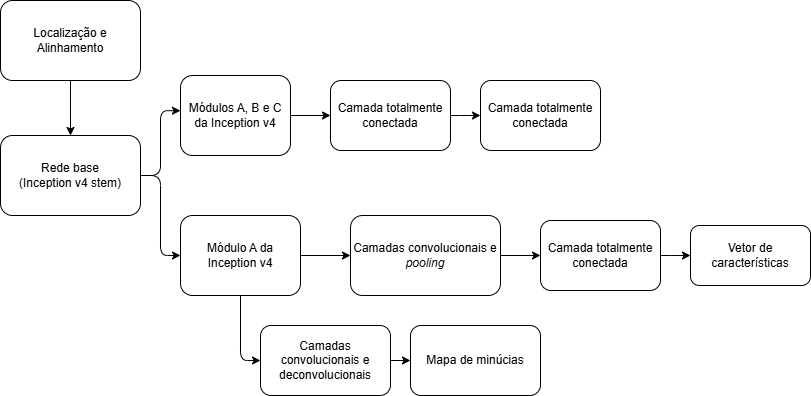
\includegraphics[width=0.8\textwidth]{diagrama-deepprint.png}
    \caption{Arquitetura da rede neural \textit{DeepPrint}}
    \label{fig:deepprint-arch}
\end{figure}

\subsubsection{Arquitetura do FLARE}\label{subsubsec:flare-arch}

O FLARE é um framework de identificação e verificação de impressões digitais baseado em uma rede neural profunda que foi treinada para extrair uma representação na forma de um tensor tridimensional após um pré-processamento que envolve alinhamento, realce e segmentação, também realizados por redes neurais profundas treinadas de forma independente.

Inicialmente a imagem passa por uma etapa de alinhamento que utiliza duas técnicas complementares, uma baseada em regressão~\cite{fingerprint_pose_via_regression} e outra baseada em votos~\cite{fingerprint_pose_via_dense_voting}. A primeira faz uma estimativa da pose da digital com base no seu contorno da imagem enquanto a segunda infere com base em predições locais baseadas em representações densas das cristas.~\citeonline{flare} argumentam que o emprego de técnicas que aliam atributos globais e locais das digitais garante um alinhamento mais preciso das digitais.

Após o alinhamento a imagem é realçada por dois modelos diferentes, o~\textit{UNetEnh} e o~\textit{PriorEnh}. A~\textit{UNetEnh} e uma rede neural convolucional baseada na arquitetura U-Net~\cite{unet} para segmentação e remoção de ruídos. A rede PriorEnh, por sua vez, desempenha o papel crítico de reconstruir parcialmente a estrutura das cristas em áreas severamente danificadas ou apagadas, utilizando para isso um conhecimento prévio sobre a geometria padrão de impressões digitais de boa qualidade.

Para a extração de características,~\citeonline{flare} desenvolveram a Rede de Representação Densa de Tamanho Fixo (\textit{Fixed-length Dense Representation Network}, FDRN). A representação extraída por essa rede, diferente do~\textit{DeepPrint}, é uma representação tridimensional que codifica de forma mais natural a segmentação das impressões digitais, assim como as suas minúcias. Ela é baseada na arquitetura da rede ResNet-34~\cite{resnet-34}, com a primeira camada de Max Pooling removida para preservação de detalhes mais finos impressões digitais. De forma semelhante ao que foi proposto em~\cite{deep_print}, a rede é dividida em dois ramos para aprendizado multi-tarefa~\cite{multitask-learning}: a primeira sub-rede extrai um mapa de minúcias ao mesmo tempo que aprende a gerar uma representação de tamanho fixo que codifica informações sobre as minúcias; a segunda sub-rede extrai um mapa de segmentação que separa a impressão digital do fundo da imagem enquanto aprende a gerar uma representação de tamanho fixo com base nos padrões dos cumes da digital. A representação final é obtida ao concatenar os resultados de ambas as sub-redes

Para a verificação de impressões digitais a representação tridimensional é achatada para um vetor, e então é calculada a distância de cossenos entre as duas impressões. Devido ao processo de alinhamento e posterior concatenação das duas representações geradas, baseadas em minúcias e na segmentação, o calculo de distâncias só considera as regiões de sobreposição entre as duas digitais.


\subsection{Experimentos}\label{subsec:experimentos}

Até o momento foram realizados experimentos com um modelo pré-treinado do DeepPrint, disponibilizado por~\citeonline{Rohwedder2023}, que pode ser obtido através do link\footnote{\url{https://drive.google.com/file/d/1R9v73hFBuy0iihz7v8eDlBcGrMDmQ9TH/view?usp=drive_link}}. O repositório com o código-fonte utilizado para o treinamento do modelo está disponível públicamente no GitHub\footnote{\url{https://github.com/tim-rohwedder/fixed-length-fingerprint-extractors}}. A seguir serão descritos como foi feito treinamento o do modelo e os testes realizados.


\subsubsection{Treinamento do DeepPrint}\label{subsubsec:deepprint-training}

\citeonline{deep_print} utilizaram o conjunto de dados longitudinal~\cite{longitudinal} de cerca de $455000$ imagens de $38291$ dedos, que não está disponível publicamente. Os autores não disponibilizaram nenhum código-fonte ou modelo pré-treinado. Dessa forma, optamos por utilizar a implementação da arquitetura do DeepPrint e modelo pré-treinado de~\citeonline{Rohwedder2023}, que tinha como objetivo avaliar o desempenho preditivo do modelo em imagens coletadas com outros tipos de sensores e com representações de tamanhos diferentes.

Com o intuito de eliminar a necessidade de coletar impressões digitais ou de utilizar um conjunto de dados público os autores utilizaram o SFinGe~\cite{handbook_of_fp_recognition} para a criação de impressões digitais sintéticas. Para o treinamento, foram utilizadas 10 impressões digitais de 6000 indivíduos, e para validação 4 imagens de 2000 indivíduos, totalizando 68000 imagens. A partir deste banco de imagens foram geradas novas imagens aplicando-se rotações, reflexões e variações de brilho e contraste de forma aleatória, assim como no artigo original. Uma outra diferença em relação ao experimento de~\citeonline{deep_print} foi o tamanho da representação. O modelo pré-treinado gera representações de 512 dimensões, com 256 de dimensões em cada sub-rede.

\subsubsection{Treinamento do FLARE}\label{subsubsec:flare-training}

Em~\cite{flare} é explicado como cada um dos módulos do~\textit{framework} FLARE foi treinado, e quais conjuntos de imagens foram utilizados em cada etapa do treinamento. Nesta seção será descrito brevemente o processo de treinamento das redes neurais que compõem o FLARE.

Os módulos de alinhamento por regressão global direta~\cite{fingerprint_pose_via_regression} e votação local densa~\cite{fingerprint_pose_via_dense_voting} foram treinados seguindo os métodos originalmente descritos por seus respectivos autores. Foram utilizadas imagens do conjunto de dados do~\textit{Diverse Pose Fingerprint} (DPF) e as primeiras 3200 imagens do NIST SD14. Para tornar a rede de alinhamento tolerante a ruídos de fundo foi empregada uma estratégia de aumento de dados que insere de forma aleatória padrões de interferência extraídos do conjunto de imagens MSRA-TD500.

Para o treinamento da~\textit{UNetEhn} também foi treinada utilizando imagens de alta resolução e suas respectivas cópias com desfoque gaussiano, padrões de linhas, caracteres manuscritos do MNIST e sobreposições de fundo do conjunto de dados BID. Já o treinamento da rede PriorEnh é estruturado em duas etapas independentes e consecutivas. Primeiro, um~\textit{autoenconder} variacional quantizado vetorial (VQ-VAE)\cite{vq-vae} é treinado de forma não supervisionada para auto-reconstruir imagens de alta qualidade do DPF. Através deste processo de aprendizado discreto, a rede cria um dicionário latente ($C$) composto por 4096 códigos com dimensão de incorporação ($d_c$) igual a 33. Esse codebook funciona como uma biblioteca geométrica que armazena estruturas de cristas limpas e regulares.

Na segunda etapa de treinamento da PriorEnh, o dicionário de padrões geométricos e o decodificador obtidos na fase anterior são congelados. Em seguida, um codificador seguindo a arquitetura do U-Net, um indexador~\textit{GatedPixelCNN}\cite{pixel-cnn} e um módulo de transformação de características (CFT)\cite{cft} são treinados conjuntamente para receber imagens com degradações simuladas e reconstruir suas versões limpas de alta qualidade.

Para o treinamento da FDRN foram utilizados os primeiros 24000 pares de impressões digitais de alta qualidade do NIST SD14 e 2.676 impressões planas de 633 dedos distintos, juntamente com suas respectivas máscaras de segmentação, foram selecionadas do DPF com o intuito de simular impressões digitais incompletas e parciais por meio da aplicação de máscaras binárias.


\subsubsection{Testes com o modelo pré-treinado}\label{subsubsec:deepprint-testing}

Até o momento foram realizados testes utilizando os conjuntos de dados do FVC2004. São 4 conjuntos de imagens divididos em parte A com 800 imagens (100 dedos com 8 impressões cada) e parte B com 80 imagens (10 dedos com 8 impressões cada).. Para aumentar a acurácia do modelo as imagens passaram por um refinamento utilizando filtros de Gabor~\cite{gabor-wavelet-transform} e redimensionamento para o tamanho adequado para a CNN.

Em seguida, as imagens são processadas pelo modelo pré-treinado, que extrai os vetores de características de ambas as sub-redes, e a similaridade por cossenos é utilizada para calcular uma pontuação. A imagem de cada dedo é comparada com as demais imagens do mesmo dedo e com todas as imagens outros dedos.

Para calcular a FNMR, FMR e EER é necessário definir um limiar de corte que a pontuação deve atingir. Foram testados os valores $[.5, .55, .6, .65, .7, .75, .8, .85, .9, .95]$.
